\documentclass[tikz,border=2mm]{standalone}
\usepackage{tikz}
\usetikzlibrary{shapes.geometric, arrows, shapes.gates.logic.US}

\definecolor{mycolor}{RGB}{0, 153, 255}
\tikzstyle{process} = [rectangle, rounded corners,
                       minimum width=2cm, minimum height=1cm,
                       text centered, draw=black, fill=mycolor,
                       text=white, line width=0.3mm]
                       
\tikzstyle{mux} = [trapezium,trapezium angle=80,trapezium stretches=true, rotate=-90, minimum width=1.5cm,  draw]

\tikzstyle{arrow} = [thick,->,>=stealth]

%defining the incrementer
\tikzset{
    pics/incrementer/.style args={#1,#2,#3}{ % 1# is name of figure, 2# is name written in ALU, #3 is node options
        code={%     x    y         x    y
            \draw (-1.65,-2.5) -- (-1.65,-0.5) -- % Left bottom straight line
                  (-1.0 , 0  ) -- (-1.65, 0.5) -- % Left second diagonal line
                  (-1.65, 2.5) -- ( 1.65, 1.5) -- % Middle downgoing diagonal line
                  ( 1.65,-1.5) -- (-1.65,-2.5);   % Middle up going diagonal line
            \node [#3] () at (0,0) {\textbf{#2}}; 
            \node [anchor=south](#1) at (-4,4) {};
%            \draw [arrow, line width=0.2mm] (-4.03,4) -- (0,4);
%            \draw [arrow, line width=0.2mm] (-2,1) node[anchor=east] {4} -- (0,1);
        }
    }
}

\begin{document}
    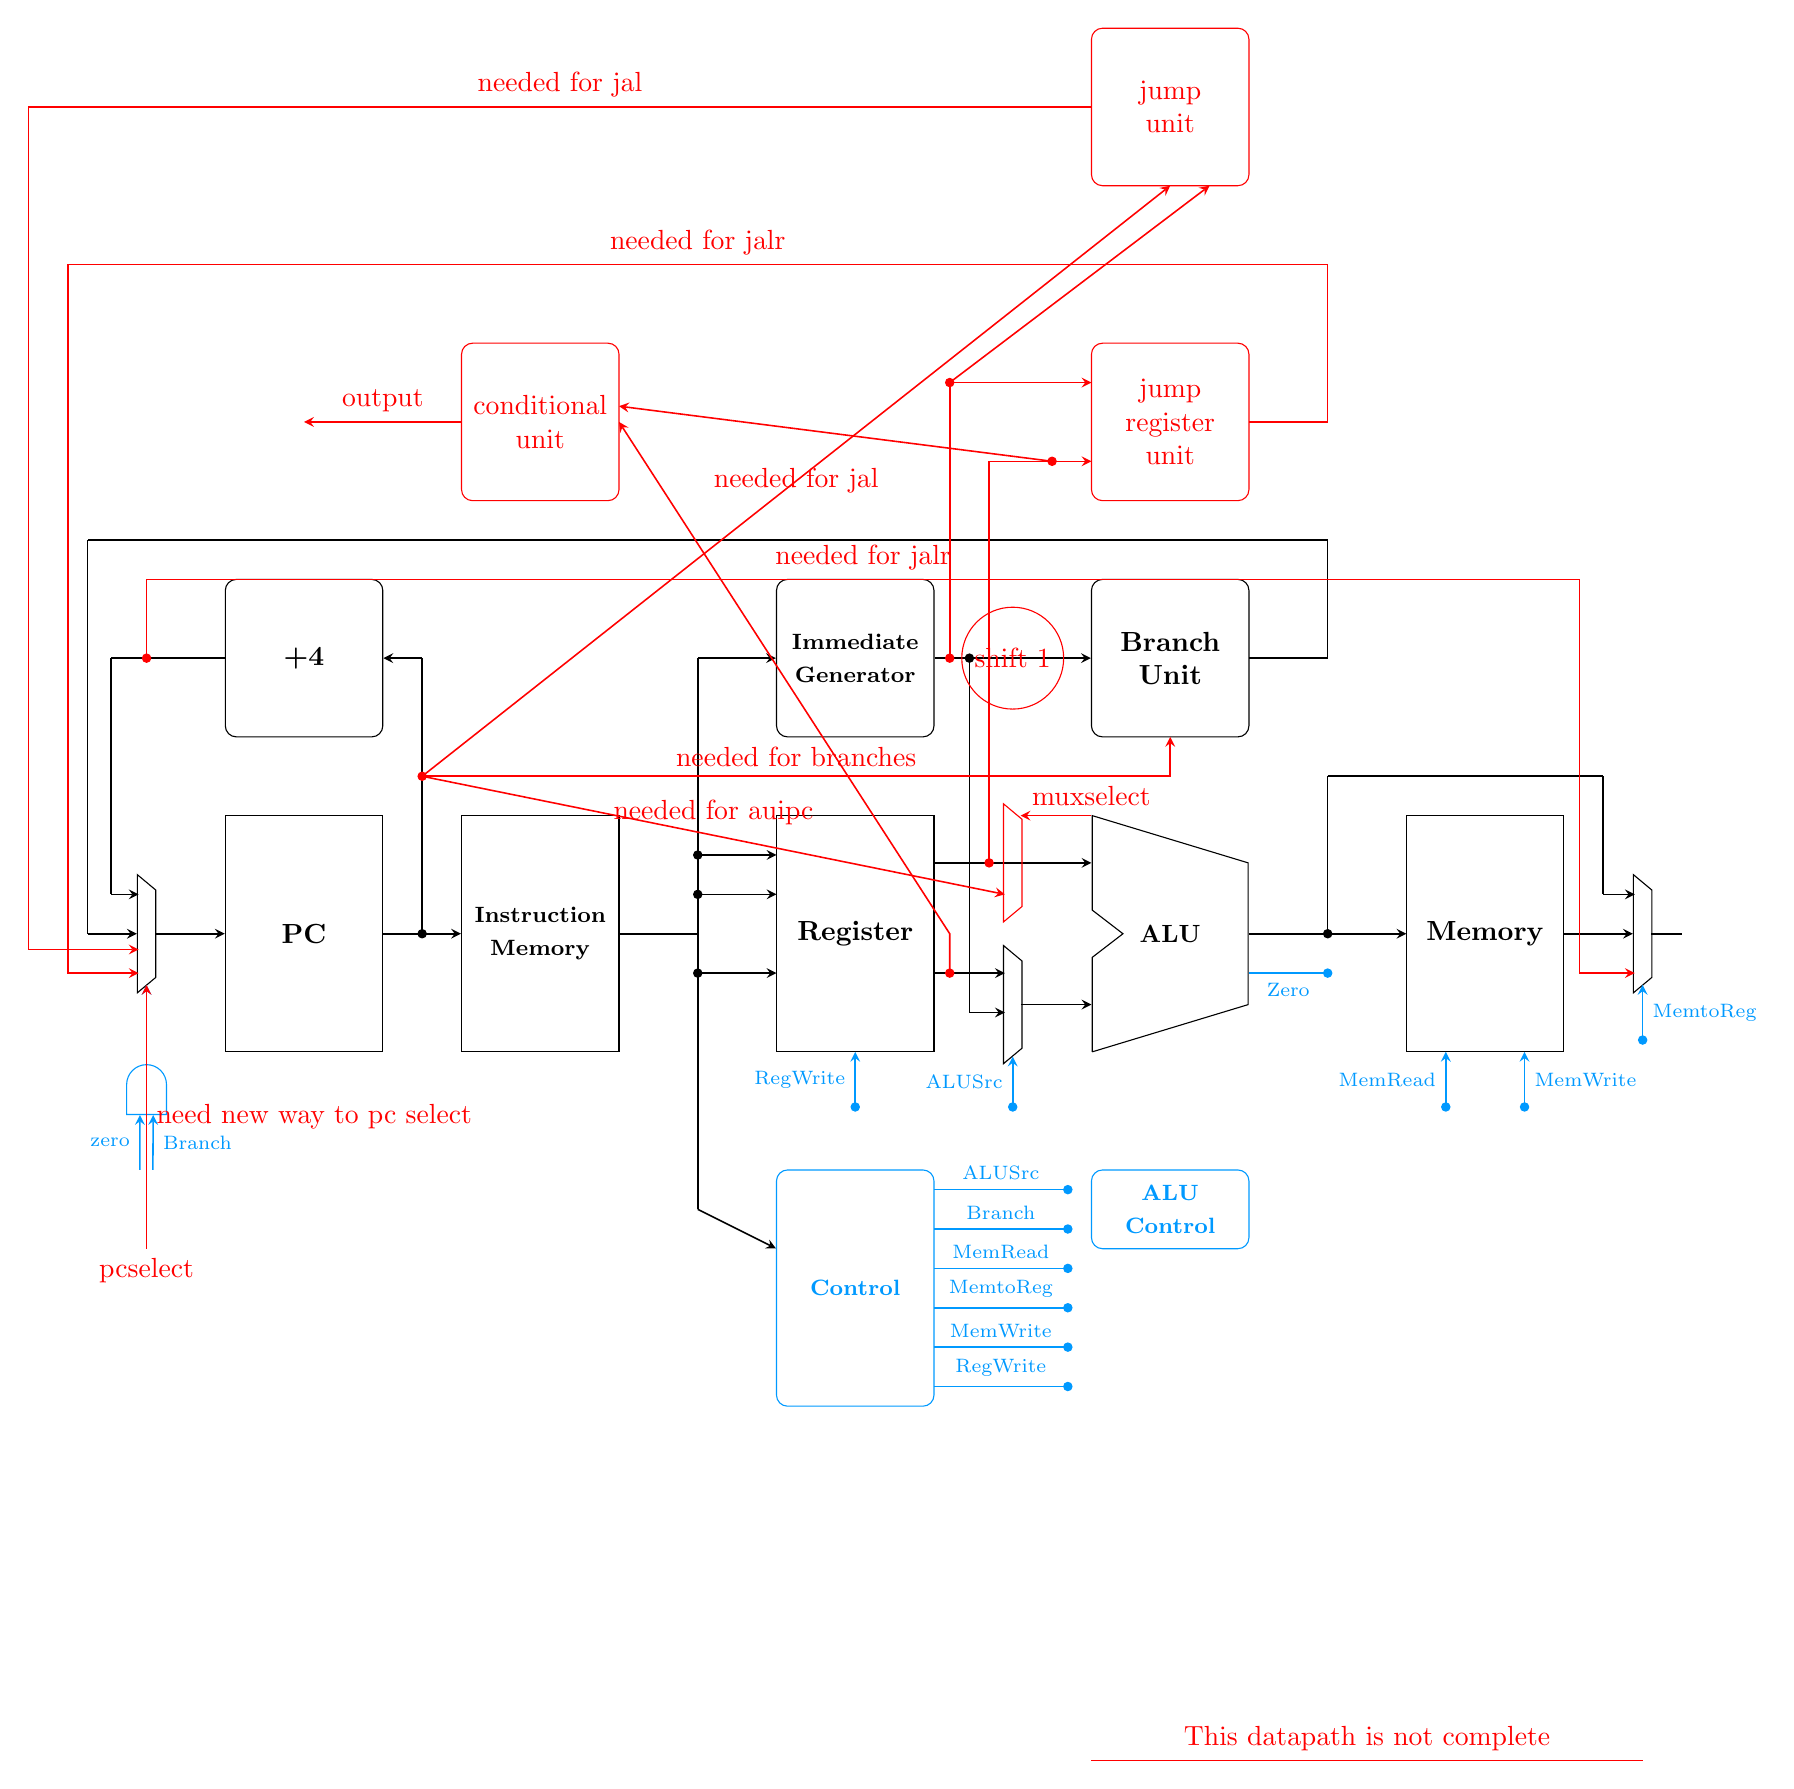
\begin{tikzpicture}[node distance=2cm]
        %First mux
        \node at (1,0) [mux] (mux1) {};
        %PC
        \node at (3,0) [rectangle, minimum width=2cm, minimum height=3cm, draw] (PC) {\textbf{PC}};
        %incrementer
        \node at (3,3.5) [rectangle, rounded corners, minimum width=2cm, minimum height=2cm, align=center, draw] (inc) {\textbf{+4}};
        %Instruction memory
        \node at (6,0) [rectangle, minimum width=2cm, minimum height=3cm, align=center,draw] (IM) {\footnotesize \textbf{Instruction}\\\footnotesize \textbf{Memory}};
        
        \draw [arrow, line width=0.2mm] (mux1) -- (PC);
        \filldraw[black] (4.5,0) circle (1.5pt); 
        \draw [arrow, line width=0.2mm] (PC) -- (IM);
        \draw [line width=0.2mm] (4.5,0) -- (4.5,3.5);
        \draw [arrow, line width=0.2mm] (4.5,3.5) -- (inc);
        
        \draw [line width=0.2mm] (inc) -- (0.55,3.5);
        \draw [line width=0.2mm] (0.55,3.5) -- (0.55,0.5);
        \draw [arrow,line width=0.2mm] (0.55,0.5) -- (0.9,0.5);
        

        %----------------------------------------------------------------------------------
        %Register
        \node at (10,0) [rectangle, minimum width=2cm, minimum height=3cm, align=center,draw] (Reg) {\textbf{Register}};
        %Immediate Generator
        \node at (10,3.5) [rectangle, rounded corners, minimum width=2cm, minimum height=2cm, align=center, draw] (immgen) {\footnotesize\textbf{Immediate}\\\footnotesize\textbf{Generator}};
        %Control
        \node at (10,-4.5) [rectangle, rounded corners, minimum width=2cm, minimum height=3cm, align=center, color=mycolor, draw] (control) {\footnotesize\textbf{Control}};
        
        \draw [line width=0.2mm] (7,0) -- (8,0);
        \draw [line width=0.2mm] (8,-3.5) -- (8,3.5);
        
        \filldraw[black] (8,1) circle (1.5pt); 
        \draw [arrow,line width=0.2mm] (8,1) -- (9,1);
        \filldraw[black] (8,0.5) circle (1.5pt);
        \draw [arrow,line width=0.2mm] (8,0.5) -- (9,0.5);
        \filldraw[black] (8,-0.5) circle (1.5pt);
        \draw [arrow,line width=0.2mm] (8,-0.5) -- (9,-0.5);
        
        \draw [arrow,line width=0.2mm] (8,3.5) -- (immgen);
        \draw [arrow,line width=0.2mm] (8,-3.5) -- (control);
        
        %----------------------------------------------------------------------------------
        %Second mux
        \node at (12,-0.9) [mux] (mux2) {};
        %ALU
        \draw    (14,0) pic[scale=0.6]{incrementer={ALU,ALU,scale=0.9}};
        %Branch unit
        \node at (14,3.5) [rectangle, rounded corners, minimum width=2cm, minimum height=2cm, align=center, draw] (bran) {\textbf{Branch}\\\textbf{Unit}};
        %ALU Control
        \node at (14,-3.5) [rectangle, rounded corners, minimum width=2cm, minimum height=1cm, align=center, color=mycolor, draw] (alucon) {\footnotesize\textbf{ALU}\\\footnotesize\textbf{Control}};
        
        %from register to alu
        \draw [arrow,line width=0.2mm] (11,0.9) -- (13,0.9);
        \draw [arrow,line width=0.2mm] (11,-0.5) -- (11.9,-0.5);
        \draw [arrow,line width=0.2mm] (12.11,-0.9) -- (13,-0.9);
        
        \draw [arrow,line width=0.2mm] (immgen) -- (bran);
        \filldraw[black] (11.45,3.5) circle (1.5pt);
        \draw [line width=0.2mm] (11.45,3.5) -- (11.45,-1);
        \draw [arrow,line width=0.2mm] (11.45,-1) -- (11.9,-1);
        
        %from branch to first muc
        \draw [line width=0.2mm] (15,3.5) -- (16,3.5);
        \draw [line width=0.2mm] (16,3.5) -- (16,5);
        \draw [line width=0.2mm] (16,5) -- (0.25,5);
        \draw [line width=0.2mm] (0.25,5) -- (0.25,0);
        
        \draw [arrow,line width=0.2mm] (0.25,0) -- (mux1);
        
        
        %----------------------------------------------------------------------------------
        %Memory
        \node at (18,0) [rectangle, minimum width=2cm, minimum height=3cm, align=center,draw] (Mem) {\textbf{Memory}};
        
        \draw [arrow,line width=0.2mm] (15,0) -- (17,0);
        \filldraw[black] (16,0) circle (1.5pt);
        \draw [line width=0.2mm] (16,0) -- (16,2);
        \draw [line width=0.2mm] (16,2) -- (19.5,2);
        \draw [line width=0.2mm] (19.5,2) -- (19.5,0.5);
        \draw [arrow,line width=0.2mm] (19.5,0.5) -- (19.9,0.5);
        
        
        
        %----------------------------------------------------------------------------------
        %Third mux
        \node at (20,0) [mux] (mux3) {};
        \draw [arrow,line width=0.2mm] (Mem) -- (mux3);
        
        \draw [line width=0.2mm] (20.11,0) -- (20.5,0);
%        \draw [line width=0.2mm] (20.5,0) -- (20.5,-2);
%        \draw [line width=0.2mm] (20.5,-2) -- (8.5,-2);
%        \draw [line width=0.2mm] (8.5,-2) -- (8.5,-1);
%        \draw [arrow,line width=0.2mm] (8.5,-1) -- (9,-1);
        
%        \draw (0,-0) -- (20,-0);

        %----------------------------------------------------------------------------------
        % Control lines
        \draw [arrow,line width=0.2mm,color=mycolor] (10,-2.2) --node[left]{\scriptsize RegWrite} (10,-1.5);
        \filldraw[mycolor] (10,-2.2) circle (1.5pt);
        \draw [arrow,line width=0.2mm,color=mycolor] (12,-2.2) --node[left]{\scriptsize ALUSrc} (12,-1.56);
        \filldraw[mycolor] (12,-2.2) circle (1.5pt);
        \draw [arrow,line width=0.2mm,color=mycolor] (17.5,-2.2) --node[left]{\scriptsize MemRead} (17.5,-1.5);
        \filldraw[mycolor] (17.5,-2.2) circle (1.5pt);
        \draw [arrow,line width=0.2mm,color=mycolor] (18.5,-2.2) --node[right]{\scriptsize MemWrite} (18.5,-1.5);
        \filldraw[mycolor] (18.5,-2.2) circle (1.5pt);
        \draw [line width=0.2mm,color=mycolor] (15,-0.5) --node[below]{\scriptsize Zero} (16,-0.5);
        \filldraw[mycolor] (16,-0.5) circle (1.5pt);
        \draw [arrow,line width=0.2mm,color=mycolor] (20,-1.35) --node[right]{\scriptsize MemtoReg} (20,-0.65);
        \filldraw[mycolor] (20,-1.35) circle (1.5pt);
        
        \draw [-,line width=0.2mm,color=mycolor] (11,-3.25) -- node[above]{\scriptsize ALUSrc} (12.7,-3.25);
        \filldraw[mycolor] (12.7,-3.25) circle (1.5pt);
        \draw [-,line width=0.2mm,color=mycolor] (11,-3.75) -- node[above]{\scriptsize Branch} (12.7,-3.75);
        \filldraw[mycolor] (12.7,-3.75) circle (1.5pt);
        \draw [-,line width=0.2mm,color=mycolor] (11,-4.25) -- node[above]{\scriptsize MemRead} (12.7,-4.25);
        \filldraw[mycolor] (12.7,-4.25) circle (1.5pt);
        \draw [-,line width=0.2mm,color=mycolor] (11,-4.75) -- node[above]{\scriptsize MemtoReg} (12.7,-4.75);
        \filldraw[mycolor] (12.7,-4.75) circle (1.5pt);
        \draw [-,line width=0.2mm,color=mycolor] (11,-5.25) -- node[above]{\scriptsize MemWrite} (12.7,-5.25);
        \filldraw[mycolor] (12.7,-5.25) circle (1.5pt);
        \draw [-,line width=0.2mm,color=mycolor] (11,-5.75) -- node[above]{\scriptsize RegWrite} (12.7,-5.75);
        \filldraw[mycolor] (12.7,-5.75) circle (1.5pt);
        
        \node at (1,-2) [and gate US, rotate=90, color=mycolor, logic gate inputs=nn,draw](and) {};
        \draw [arrow,line width=0.2mm,color=mycolor] (and.output) -- (1,-0.65);
        \draw [arrow,line width=0.2mm,color=mycolor] (0.914,-3) --node[left]{\scriptsize zero} (and.input 1);
        \draw [arrow,line width=0.2mm,color=mycolor] (1.08,-3) --node[right]{\scriptsize Branch} (and.input 2);
        %----------------------------------------------------------------------------------
        % New stuff
        \node at (12,3.5) [circle, color=red, draw] {shift 1};
        \draw [arrow,line width=0.2mm, color=red]  (1,3.5) -- (1,4.5) --node[above]{needed for jalr} (19.2,4.5) -- (19.2, -0.5) -- (19.9,-0.5);
        \filldraw[red] (1,3.5) circle (1.5pt);
        \draw [arrow,line width=0.2mm, color=red] (4.5,2) --node[above]{needed for branches} (14,2) -- (14,2.5);
        \filldraw[red] (4.5,2) circle (1.5pt);
        
        %jump register unit
        \node at (14,6.5) [rectangle, color=red, minimum width=2cm, minimum height=2cm, rounded corners, align=center, draw] {jump \\ register \\ unit};
        %jump unit
        \node at (14,10.5) [rectangle, color=red, minimum width=2cm, minimum height=2cm, rounded corners, align=center, draw] {jump \\ unit};
        
        %rs1 to jump register
        \draw [arrow,line width=0.2mm, color=red] (11.7,0.9) -- (11.7,6) -- (13, 6);
        \filldraw[red] (11.7,0.9) circle (1.5pt);
        %immgen to jump reigster
        \draw [arrow,line width=0.2mm, color=red] (11.2,3.5) -- (11.2,7) -- (13, 7);
        \filldraw[red] (11.2,3.5) circle (1.5pt);
        %jump to first mux
        \draw [arrow,line width=0.2mm, color=red] (15,6.5) -- (16,6.5) -- (16, 8.5) --node[above]{needed for jalr} (0, 8.5) -- (0,-0.5) -- (0.9,-0.5);
        
        %pc select
        \draw [arrow,line width=0.2mm, color=red] (1,-4)node[below]{pcselect} --node[right]{need new way to pc select} (1,-0.65);
        %conditional unit
        \node at (6,6.5) [rectangle, color=red, minimum width=2cm, minimum height=2cm, align=center, rounded corners, draw] {conditional \\ unit};
        %rs2 to conditional unit
        \draw [arrow,line width=0.2mm, color=red] (11.2,-0.5) -- (11.2, 0) -- (7, 6.5);
        \filldraw[red] (11.2,-0.5) circle (1.5pt);
        %rs1 to conditional unit
        \draw [arrow,line width=0.2mm, color=red] (12.5,6) -- (7, 6.7);
        \filldraw[red] (12.5,6) circle (1.5pt);
        %conditional unit output
        \draw [arrow,line width=0.2mm, color=red] (5,6.5) --node[above]{output} (3, 6.5);
        
        %pc to mux new
        \draw [arrow,line width=0.2mm, color=red] (4.5,2) --node[above]{needed for auipc} (11.9, 0.5);
        %mux new select
        \draw [arrow,line width=0.2mm, color=red] (13, 1.5)node[above]{muxselect} -- (12.1, 1.5);
        %new mux
        \node at (12,0.9) [mux, color=red] (newmux) {};
        %pc to jump unit
        \draw [arrow,line width=0.2mm, color=red] (4.5,2) --node{needed for jal} (14,9.5);
        %immgen to jump unit
        \draw [arrow,line width=0.2mm, color=red] (11.2,7) -- (14.5, 9.5);
        \filldraw[red] (11.2,7) circle (1.5pt);
        %jump unit to mux 1
        \draw [arrow,line width=0.2mm, color=red] (13,10.5) --node[above]{needed for jal} (-0.5, 10.5) -- (-0.5,-0.2) -- (0.9,-0.2);
        
        \draw [line width=0.2mm, color=red] (13,-10.5) --node[above]{This datapath is not complete} (20, -10.5);
        
    \end{tikzpicture}
\end{document}
